% !TeX encoding = UTF-8
% !TeX spellcheck = en_US
% !TeX root = presentation.tex

\subsection{Simulation}

\begin{frame}{Simulation}
    \begin{itemize}
        \item Simple Two Dimensional Robot Simulator(STDR)	
        \item Tasks  performed:
        \begin{itemize}
            \item Map Building
            \item Localization
        \end{itemize}
    \end{itemize}
    
    \centering
    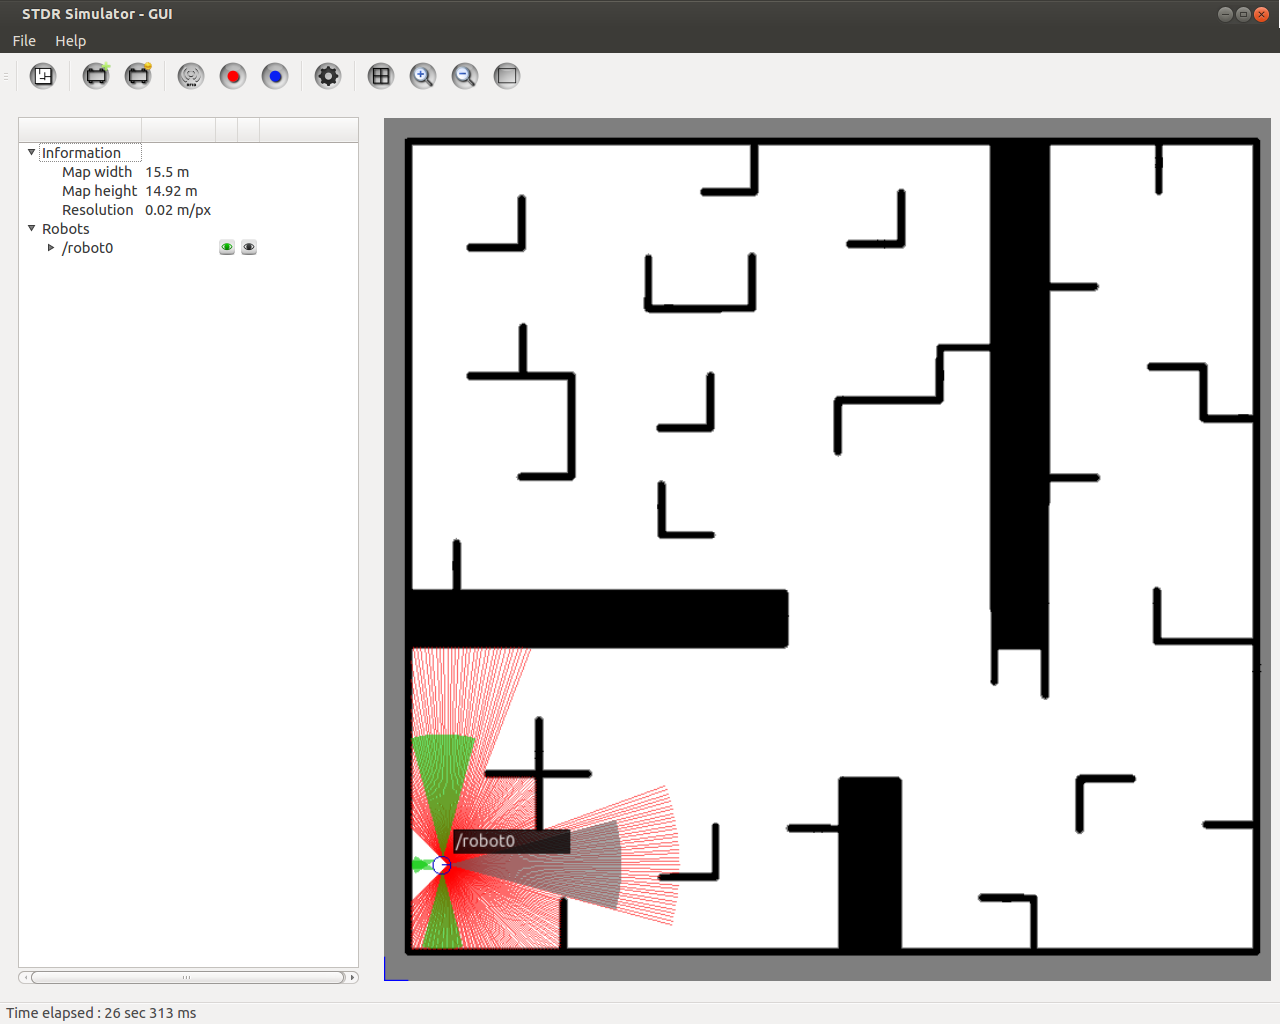
\includegraphics[width=90mm,height=55mm]{gfx/stdr_simulator}
    
\end{frame}
\begin{frame}{Map building I}
    \begin{itemize}
        \item Gmapping is used to build the map
        \begin{itemize}
            \item Uses laser scanner 
        \end{itemize}
        \item Map Server
        \begin{itemize}
            \item Provides map saver utility, to save generated map in files(yaml and pgm)
            \item Offers map data as a ROS Service
        \end{itemize}
        
    \end{itemize}
\end{frame}
\begin{frame}{Localization I}
    \begin{itemize}
        \item Adaptive Monto Carlo Localization(AMCL) is used to localize the robot
        \item Uses particle filter to track the pose of robot
        \item What it needs?
        \begin{itemize}
            \item Laser scans
            \item Initial pose
            \item Transforms
            \item Map 
        \end{itemize}
    \end{itemize}
\end{frame}